\section{Dynamical SIR Benchmark: PCI on Continuous Outcomes}\label{sec:sir_benchmark}

The actual-causality benchmark of Section~\ref{sec:ac_benchmark} exercises the
necessity-only specialisation of \ourapproach on a discrete outcome with a
closed-form ground truth. This section shifts to the regime where AC has no
verdict to compare against: a Bayesian dynamical model with a continuous
outcome and asymmetrically interacting causes. The benchmark mirrors a public
chirho tutorial%
\footnote{\url{https://basisresearch.github.io/chirho/explainable_sir.html}}
in setup and query, which uses chirho's \texttt{SearchForExplanation} handler
to compute classical actual-cause probabilities. We keep the same model and
the same query but replace the explanatory machinery with the \ourapproach
thin-search sampler. The full implementation, raw outputs and plotting code
are in the companion notebook
\texttt{docs/source/sir\_benchmark.ipynb}.

\medskip\noindent\textit{Model.}
The dynamics are the standard SIR system
\(\dot S = -\beta S I,\, \dot I = \beta S I - \gamma I,\, \dot R = \gamma I\),
with Bayesian priors $\beta\sim\mathrm{Beta}(18,600)$ and
$\gamma\sim\mathrm{Beta}(1600,1600)$. Two non-pharmaceutical policies, each
enacted with prior probability $1/2$, modulate the transmission rate via an
intervention strength $l\in[0,1]$ that scales $\beta_0$ to $(1-l)\beta_0$.
Lockdown alone has efficiency $0.6$; masking efficiency depends on lockdown
($0.1$ under lockdown, $0.45$ on its own); the joint efficiency is the
clamped sum, capped at $0.95$. Lockdown is enacted at $t=1$, masking at
$t=1.5$. The outcome is the \emph{overshoot}, the peak-to-final $S$ gap
of the simulated trajectory, and the undesirable event is
$\mathrm{os\_too\_high}=\mathbbm{1}[\mathrm{overshoot}>24]$ on a $100$-person
population.

\medskip\noindent\textit{But-for analysis fails to separate the suspects.}
Conditioning on each pair of policy decisions and drawing $100$ predictives
yields $\Pr(\mathrm{overshoot}>24) \approx 0.07$ with no intervention, $0.67$
with both policies, but $0.82$ with lockdown only and $0.87$ with mask only.
The mechanism is the asymmetric joint efficiency: combining the two policies
caps the transmission reduction at $0.95$, but neither policy alone reaches
that cap, and mask-only is comparatively weak unless lockdown is absent (which
shifts mask efficiency from $0.1$ to $0.45$). But-for cannot disentangle this
context dependence: it treats each policy as a binary cause and reports an
aggregate effect, with no way to express that lockdown's causal contribution
depends on whether masking is in force. Figure~\ref{fig:sir_trajectories}
visualises the four interventional regimes: the trajectory bands collapse
toward the unintervened baseline only under both policies, while either
policy on its own leaves the infectious peak essentially intact, mirroring
the near-equal but-for overshoot probabilities.

\begin{figure}[htbp]
\centering
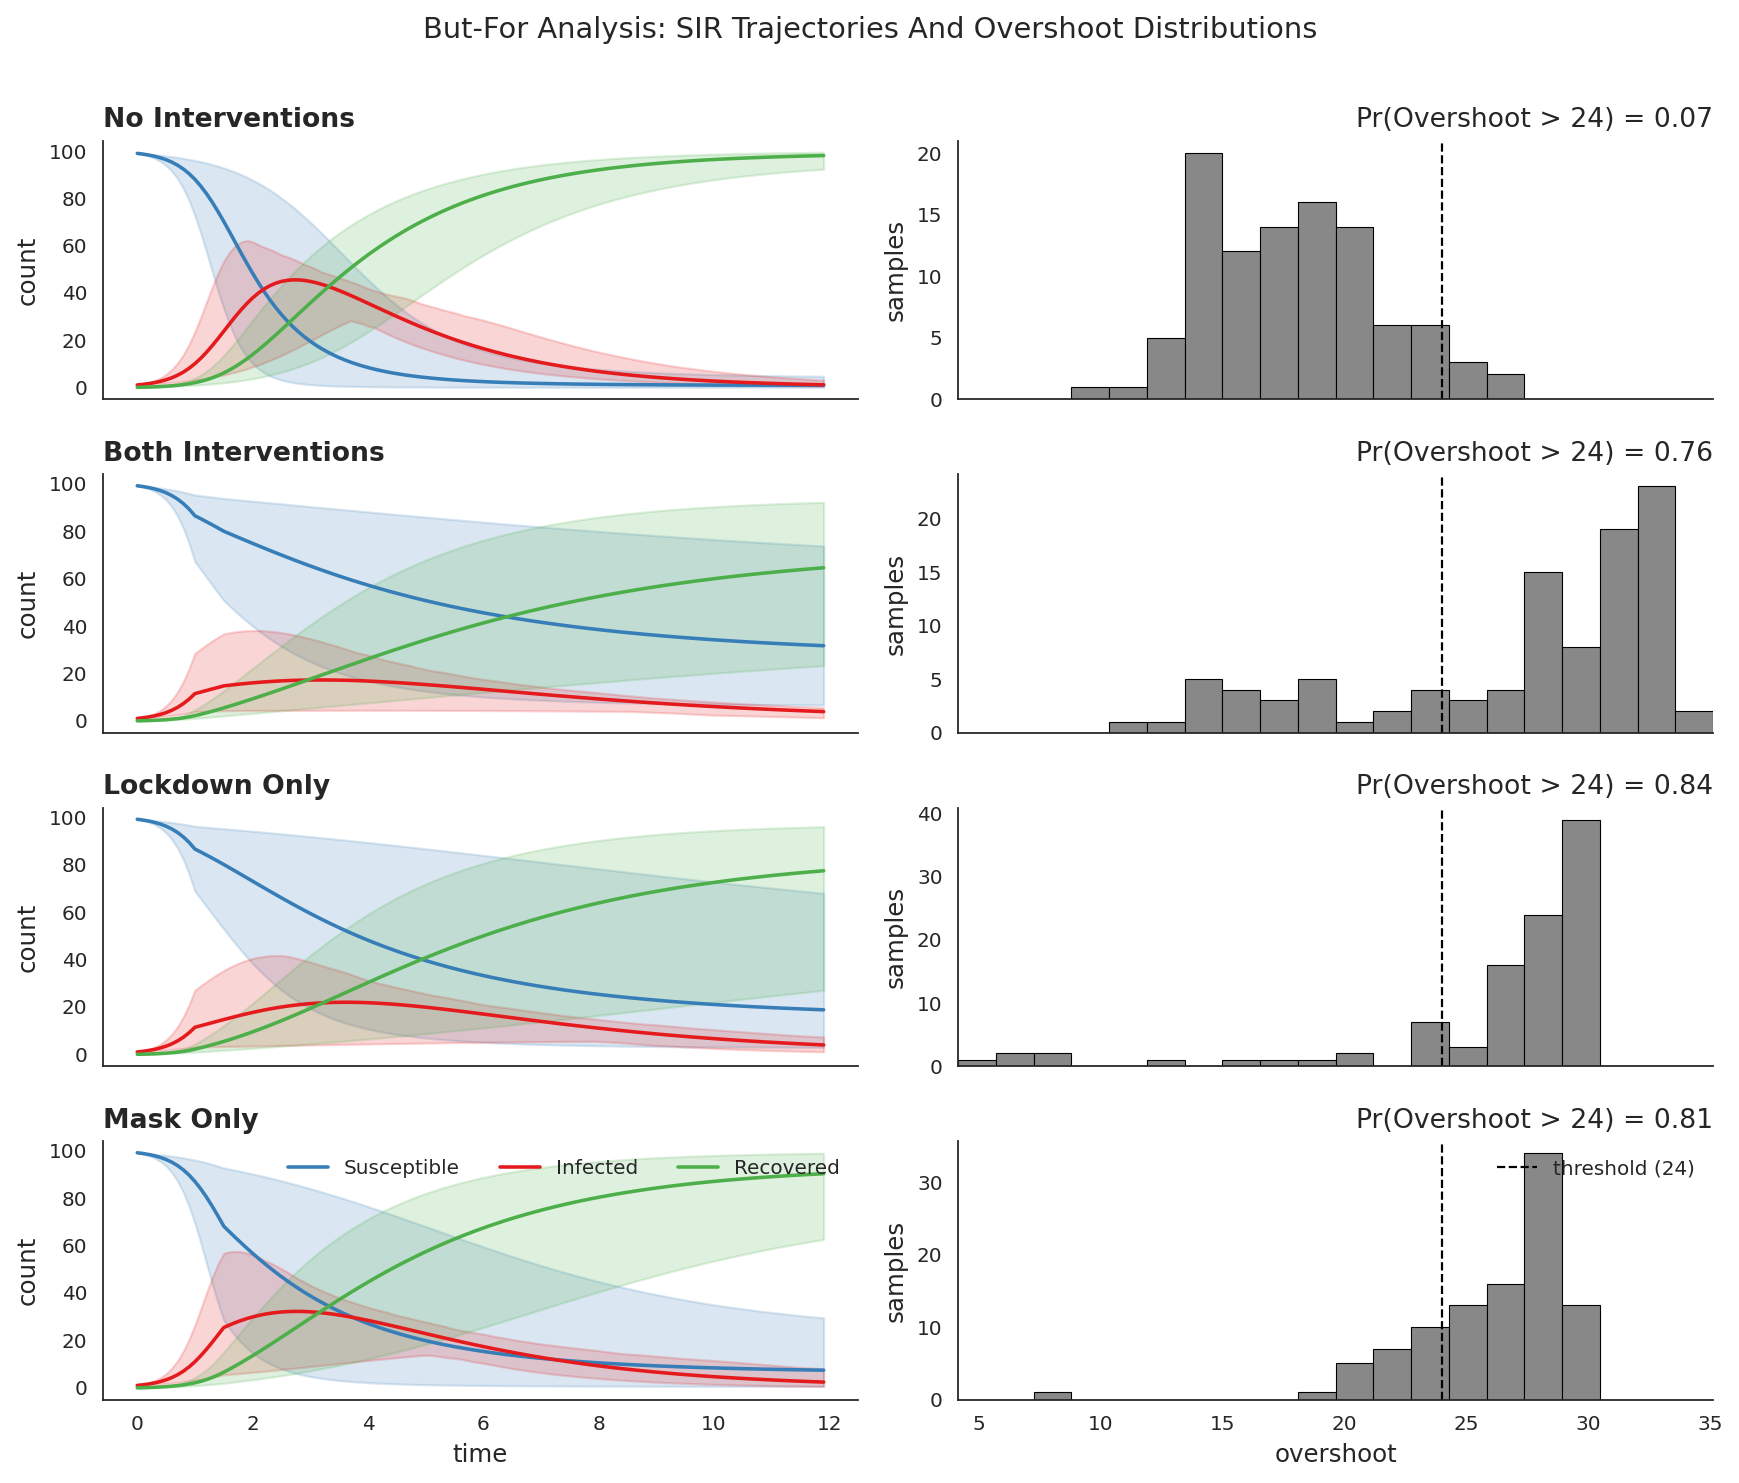
\includegraphics[width=0.92\linewidth]{docs/source/sir_benchmark/sir_butfor.png}
\caption{SIR trajectories and overshoot distributions under the four
interventional regimes (no interventions, both policies, lockdown only, mask
only). Left: posterior bands for susceptible (blue), infectious (red) and
recovered (green) over time, with the lockdown enacted at $t=1$ and the mask
mandate at $t=1.5$. Right: per-regime histograms of the overshoot, with the
$24$-overshoot threshold marked. Either policy on its own leaves the
infectious peak essentially intact; only the joint regime suppresses it
appreciably, yet the lockdown-only and mask-only overshoot probabilities are
near-indistinguishable: the asymmetric joint efficiency that
\ourapproach disentangles.}
\label{fig:sir_trajectories}
\end{figure}

\medskip\noindent\textit{\ourapproach thin-search procedure.}
The suspects are $\{\mathrm{lockdown},\mathrm{mask}\}$. The witnesses are
drawn from the policy efficiencies
$\{\mathrm{lockdown\_efficiency}, \mathrm{mask\_efficiency},
\mathrm{joint\_efficiency}\}$, with the suspect itself excluded from the
witness set on each draw. The factual world fixes both policies on
($\mathrm{lockdown}=1, \mathrm{mask}=1$), so the factual outcome
$y^\star=\mathrm{overshoot}$ is read from the same trajectory. For each
suspect the sampler draws $2{,}500$ regimes, scoring each with the
$|y^\star-y_{\mathrm{nec}}| - |y^\star-y_{\mathrm{suff}}|$ statistic and
averaging across regimes. The $\mathrm{nec}$ term rewards regimes where
removing the suspect moves the outcome \emph{away} from $y^\star$; the
$\mathrm{suff}$ term rewards regimes where fixing the suspect at factual
keeps the outcome \emph{close} to $y^\star$.

\medskip\noindent\textit{Single-world results.}
\ourapproach assigns lockdown roughly $2.0\times$ the responsibility of
mask:
\begin{center}
\small
\begin{tabular}{lccc}
\toprule
suspect & $\overline{|y^\star\!-\!y_{\mathrm{nec}}|}$ &
          $-\overline{|y^\star\!-\!y_{\mathrm{suff}}|}$ &
          total \\
\midrule
lockdown & $8.12$ & $-6.58$ & $\mathbf{1.54}$ \\
mask     & $7.43$ & $-6.67$ & $\mathbf{0.76}$ \\
\bottomrule
\end{tabular}
\end{center}
The gap is driven entirely by the necessity term: removing lockdown moves
the overshoot further from $y^\star$ than removing mask does ($8.12$ vs
$7.43$ in mean absolute distance), while the sufficiency terms agree to
within $0.1$. This is consistent with the but-for finding that either
policy \emph{alone} is roughly equally bad. What distinguishes the suspects
is that lockdown's removal \emph{under context} (with witnesses pinned to
factual) pulls the world further from $y^\star$ than mask's removal does.
Figure~\ref{fig:sir_heatmap} makes the necessity-term gap visible. Each
point is one sampled regime, with $y_{\mathrm{nec}}$ on the horizontal axis
(focal suspect intervened to alternative, other active suspects in
$\mathbf{C}\setminus\{X\}$ intervened, witnesses at factual) and
$y_{\mathrm{suff}}$ on the vertical axis (focal suspect at factual, other
active suspects intervened, witnesses at factual). The dotted red cross-hair
marks the factual outcome $y^\star$ at the both-policies-on world
($\mathrm{lockdown}=\mathrm{mask}=1$); because that world is the
high-overshoot scenario, $y^\star$ sits near the upper-right of the cloud
rather than at its centre, and a regime contributes positively to the score
iff its point lies further from the cross-hair along $x$ than along $y$.
Under that geometry the lockdown density is shifted noticeably toward
smaller $y_{\mathrm{nec}}$ at fixed $y_{\mathrm{suff}}$ --- removing
lockdown pulls $y_{\mathrm{nec}}$ well below $y^\star$ while
sufficiency-side overshoot stays close to $y^\star$ --- whereas the mask
density sits closer to the $y_{\mathrm{nec}}=y_{\mathrm{suff}}$ diagonal,
indicating that removing mask does not pull the world as far from
$y^\star$.

\begin{figure}[htbp]
\centering
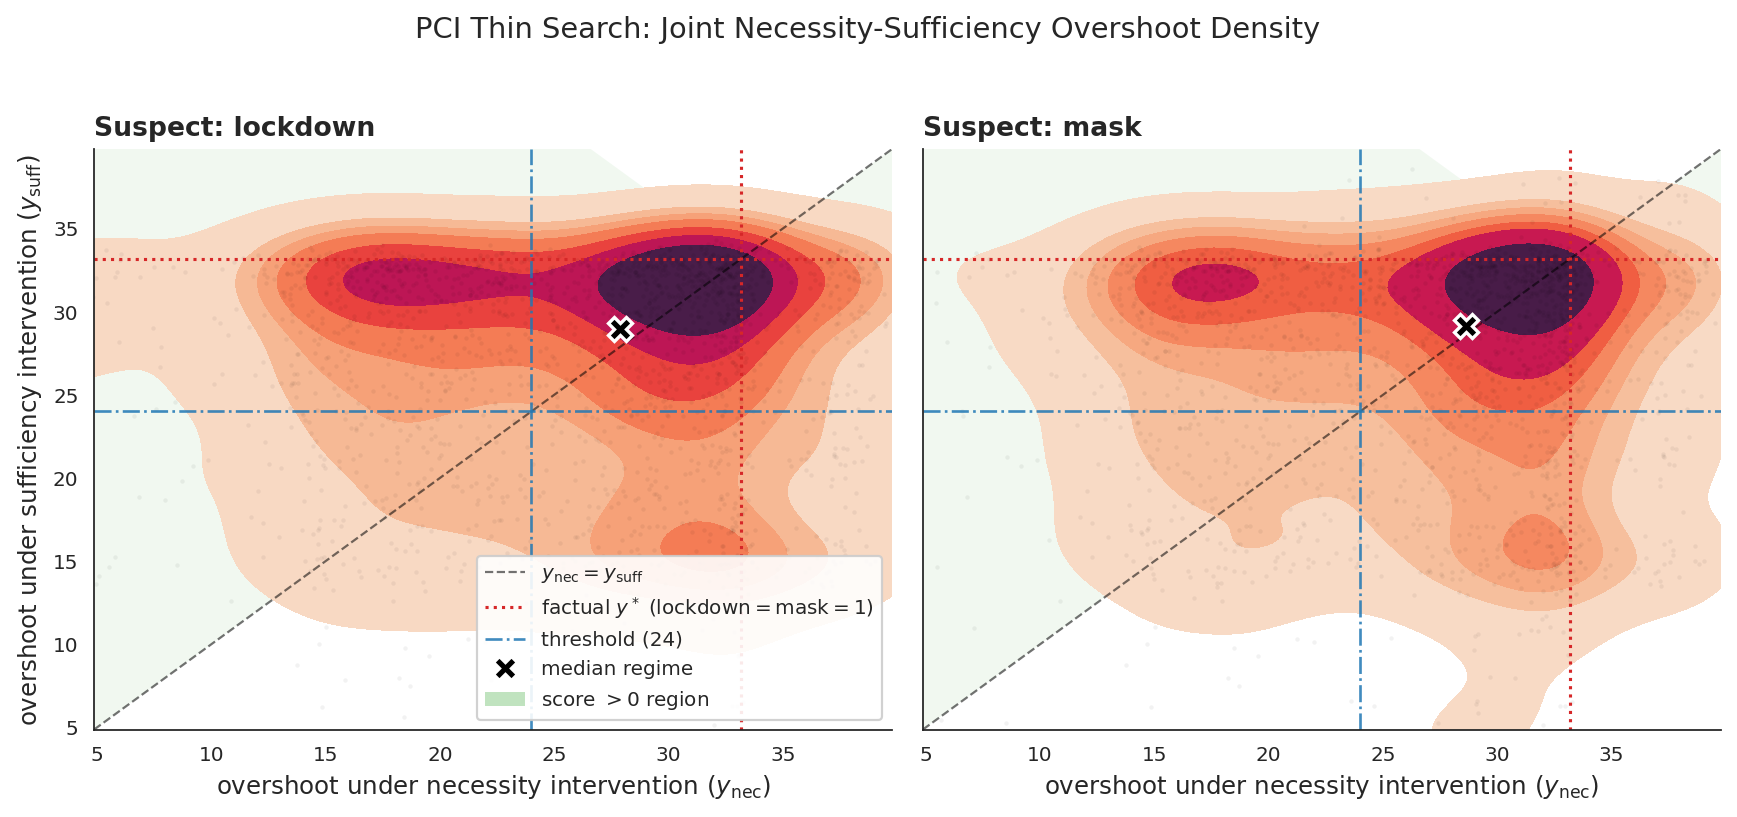
\includegraphics[width=0.92\linewidth]{docs/source/sir_benchmark/sir_heatmap.png}
\caption{Joint necessity-sufficiency overshoot density per suspect. Each
point is one sampled regime. Dotted red cross-hair: factual $y^\star$ at
$\mathrm{lockdown}=\mathrm{mask}=1$ (the high-overshoot anchor); dash-dot
blue: the $24$-overshoot threshold; dashed black:
$y_{\mathrm{nec}}=y_{\mathrm{suff}}$. A regime contributes positively to
the PCI total iff it sits further from the red cross-hair along the
necessity axis than along the sufficiency axis. The lockdown density is
shifted toward smaller $y_{\mathrm{nec}}$ relative to $y_{\mathrm{suff}}$
(the cause signature on this geometry); the mask density sits closer to
the diagonal.}
\label{fig:sir_heatmap}
\end{figure}

\medskip\noindent\textit{Robustness across factual worlds.}
We replicate the analysis across $10$ factual worlds drawn from the prior
(rather than the single hand-set world above), running thin search on each
and averaging. Lockdown's mean total exceeds mask's in the majority of
worlds; the verdict is not an artifact of the chosen factual.

\medskip\noindent\textit{Effect of context.}
The chirho tutorial isolates one downstream variable at a time, asking
whether the verdict survives when that variable is held fixed at factual
versus left free. We replicate the experiment by partitioning the
\ourapproach regimes by whether the partner-policy efficiency variable was
sampled into the witness set
(Figure~\ref{fig:sir_contexts}). For lockdown, with
$\mathrm{mask\_efficiency}$ \emph{fixed} as a witness the score is $0.81$;
\emph{free}, it rises to $2.67$. For mask, with $\mathrm{lockdown\_efficiency}$
\emph{fixed} the score is $-0.48$ (mask fails to register as a cause at
all under that context regime) and \emph{free} it rises to $2.72$.
Lockdown therefore registers as a cause in both context regimes, while
mask's status as a cause is contingent on its partner being allowed to
adapt. \ourapproach thus expresses not just \emph{which} policy is the
dominant cause but \emph{how robustly} that causal claim holds across
counterfactual contexts: a finer-grained verdict than the binary
``actual cause / not'' that classical AC produces.

\begin{figure}[htbp]
\centering
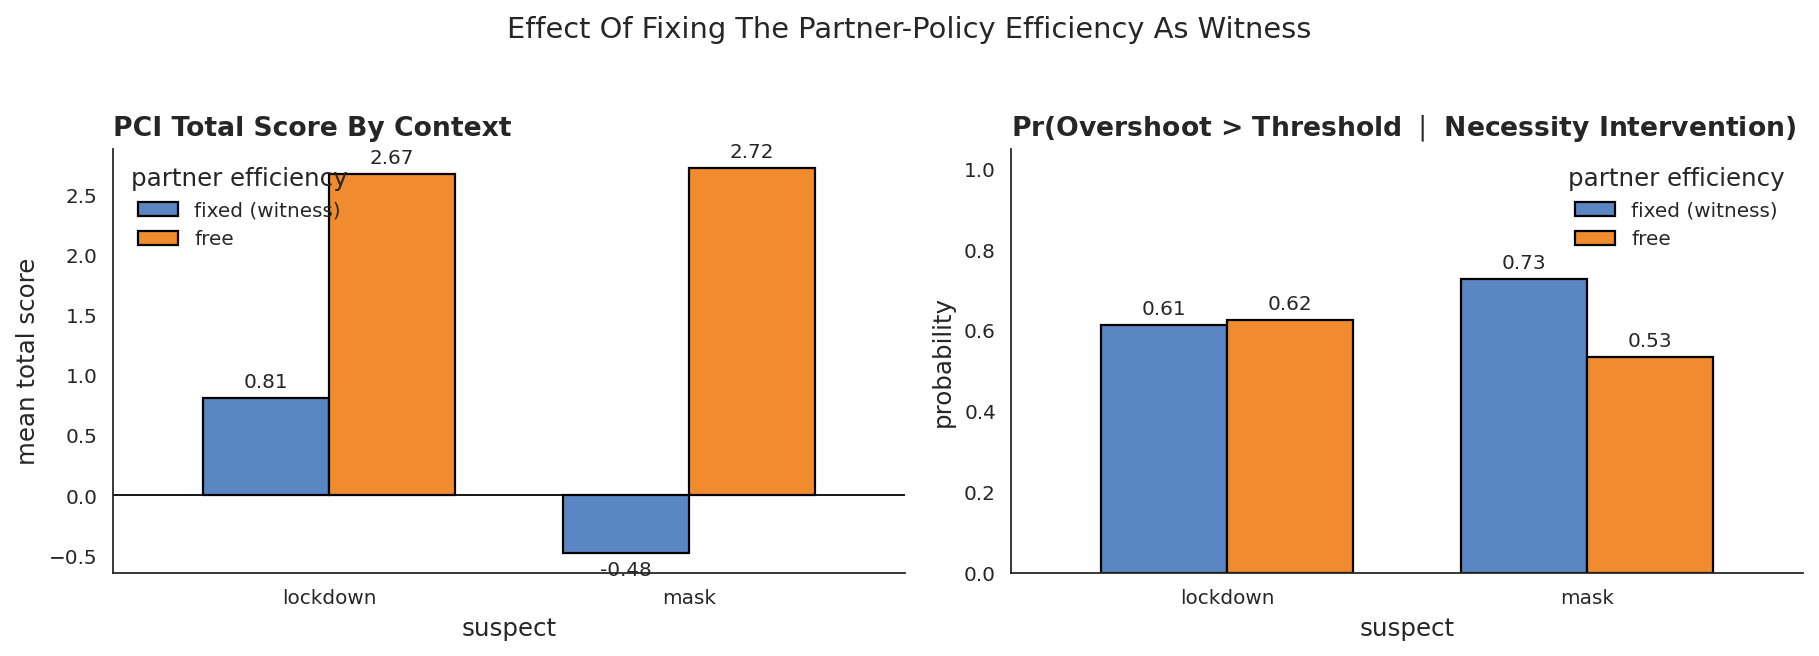
\includegraphics[width=0.92\linewidth]{docs/source/sir_benchmark/sir_contexts.png}
\caption{Different-contexts experiment. Bars compare PCI total score (left)
and $\Pr(\mathrm{overshoot}>24\mid\mathrm{necessity})$ (right) when the
partner-policy efficiency variable is fixed as a witness versus left free.
Lockdown's score is positive in both regimes; mask's score flips sign
across regimes, indicating that mask is a context-sensitive rather than a
robust cause.}
\label{fig:sir_contexts}
\end{figure}

\medskip\noindent\textit{Takeaway.}
On the dynamical SIR setting, \ourapproach recovers the qualitative
diagnosis of the chirho tutorial --- lockdown is the proximate cause of
excessive overshoot, despite both policies appearing similar under but-for
analysis --- and expresses it on a continuous, decomposable scale. The
necessity-vs-sufficiency decomposition distinguishes suspects whose
isolation effects are similar but whose removal-under-context effects
diverge; the contexts experiment further distinguishes robust from
context-sensitive causes. The same machinery applies to any chirho
probabilistic program with a continuous outcome and a tractable enumeration
over interventional regimes.

\paragraph{Where we go next.} The SIR benchmark scales \ourapproach to a
research-grade Bayesian dynamical model and demonstrates that the joint kernel
captures patterns that AC cannot adjudicate. Section~\ref{sec:avm} pushes the
demonstration one step further: a deployed automated valuation model trained on
millions of points, with deep neural-network components and a sparse variational
GP outcome head. The question there is no longer whether \ourapproach agrees with
a known ground truth (on a proprietary production model none is available),
but whether the computation is feasible at all, and whether the qualitative
SHAP-vs-PCI divergences observed on the synthetic side persist on a real trained
system.
